
\section{Ein kurzer geschichtlicher Abriss}
Wir wollen auch einen kurzen Abriss der durchaus interessanten Geschichte der Energieübertragung mit Gleich- und Wechselspannung geben. Dabei beziehen wir uns bei der Geschichte bis in die 1980er Jahre primär auf \cite{Schymroch}.

Die Geschichte der elektrischen Energie begann 1882 auf der Internationalen Ausstellung in München – mit einer Gleichstrom-Anlage. Der französische Physiker Marcel Deprez übertrug einer elektrische Leistung von 1,4 kW von Miesbach nach München – also über 57 km – mit zwei einfachen Telegrafendrähten mit einer Spannung zwischen 1,5 kV und 2,0 kV. Die Demonstationsanlage betrieb in München die Pumpen eines Springbrunnens. Die Verluste der Anlage betrugen 78\%. Eine weitere Steigerung der Spannung auf 6 kV scheiterte an Isolationsschwierigkeiten beim Gleichstrom-Generator. Dieses Problem wurde 1884 von Lafontaine gelöst, indem mehrere von einander isoliert montierte Generatoren parallelgeschalten wurden und auch auf der Verbraucher-Seite wurden parallelgeschaltene Motoren verwendet. Dadurch konnte der Wirkungsgrad einer 50\ km langen Leitung auf 50\% erhöht und 70\ kW übertragen werden.

Auch nach Entdeckung des Transformators im Jahr darauf, wurde Wechselspannung -- obwohl sie sich verlustarm hochspannen ließ -- weiterhin nicht verwendet.
Dies ist auf den zur damaligen Zeit sehr renommierten italenischen Physiker Galileo Ferraris zurückführen,
der einen falschen, aber sehr überzeugenden Beweis erbrachte, dass Wechselspannungsübertragungen maximal einen Wirkungsgrad von nur 50\% erreichen können.
Da dem Beweis des berühmten Physikers glauben geschenkt wurde, wurde vorübergehend nicht an dem Thema weitergearbeitet.
Auch die Demonstration einer Drehstrom-Übertragung von Laufen nach Frankfurt auf der dortigen Weltausstellung im Jahr 1891 konnten die Favorisierung der Gleichstromübertragung nicht stoppen.
Der Schweizer Ingenieur René Thury -- auch bekannt als der König des Gleichstroms -- hatte ein wirksames und zuverlässiges Regelungssystem für die in Reihe geschalteten Generatoren und Motoren entwickelt, so dass Gleichstrom mit Spannungen von bis zu 180\ kV übertragen werden konnte. In den nächsten zwanzig Jahren wurden 15 Übertragungen nach dem Prinzip von Thury gebaut. Das letzte dieser Anlagen und gleichzeitig auch das letzte Gleichspannungssystem mit mechanischen Wandlern war die Anlage zwischen Moutiers und Lyon, sowie später den Zwischenstationen Rosiers und Vignotanne. Sie Übertrug zunächst 4,5\ MW und nach einem Ausbau 14\ MW Leistung. Die Anlage bestand aus drei Kraftwerken und zwei Verbraucherstationen (eine eigene für die Straßenbahnen), war also vergleichsweise komplex. Die Anlage wurde 1937 zugunsten einer, der ab 1930 als überlegen angesehenen, DHÜ-Systeme demontiert. Die Idee der HGÜ geriet jedoch nicht in Vergessenheit, da zu jener Zeit mit den Stromrichtern die Grundlage für moderne Stromrichterstationen erfunden wurde.

Die ersten Versuchsanlagen mit, auf Thyratron-Stromrichtern, basierenden Quecksilberdampfgleichrichtern wurden in den USA entwickelt, wo 1936 eine erste 26\ km lange Versuchsanlage mit einer Leistung von 5,25\ MW bei einer Nennspannung von 30\ kV errichtet wurde. Sie wurde zwischen zwei Netzen mit unterschiedliche Frequenz (40\ Hz und 60\ Hz) gebaut um zu demonstrieren, dass die Netze nicht synchron sein müssen. Die erste Versuchsanlage in Deutschland wurde 1944 als Zwei-Leiter-Anlage mit Spannungen von $\pm 200 kV$ von der AEG und Siemens gebaut und hatte eine Leistung von 60\ MW. Nach dem Krieg wurde die Anlage von russischen Ingenieuren demontiert und zwischen Kashira und Moskau als Ein-Leiter-Versuchsanlage wieder aufgebaut.

Die erste kommerziell betriebene Anlage ist die schon angesprochene Anlage zur vollständigen Wirkleistungsversorgung der Insel Gotland mit einem 20 MW-Seekabel mit der Spannung von -100 kV.

Seit Beginn der 1970er Jahre wurden die Thyratron-Gleichrichter durch ihre halbleiteräquivalenten, den Thyristoren ersetzt. Die letzte mit Thyratrons gebaute Anlage war die englische HGÜ Kingsnorth. Thyristor-Technologie wird bis heute bei HGÜ-Stromrichtern verwendet, jedoch kam ab 1997 die IGBT-Technik (Bipolartransistor mit isolierter Gate-Elektrode) als Alternative hinzu. Derartige Anlagen werden oft auch unter den Namen HVDC light oder HVDC plus vertrieben.
Während die Leistung von IGBT-basierten Anlagen auf deutlich unter 1.000 MW beschränkt ist, gibt es bereits Thyristor-Anlagen mit Leistungen von bis zu 6.400 MW:
Die chinesische HGÜ Xianjiaba - Shanghai wurde 2010 fertiggestellt.\cite{Kao}
Sie transportiert eine Leistung von 6.400 MW bei einer Spannung von $\pm800 kV$ über 2071 Kilometer und
soll nur die erste von 12 bis 2018 fertiggestellten derartig dimensionierten Gleichstrom-Leitungen in China sein.\cite{Liste}
Die Längen der HGÜ-Leitungen betragen bis zu 2.400 Kilometer bei Freileitungen und bis zu 700 km bei Kabeln.\cite{Liste} 

\begin{figure}[htbn]
\begin{center}
\noindent
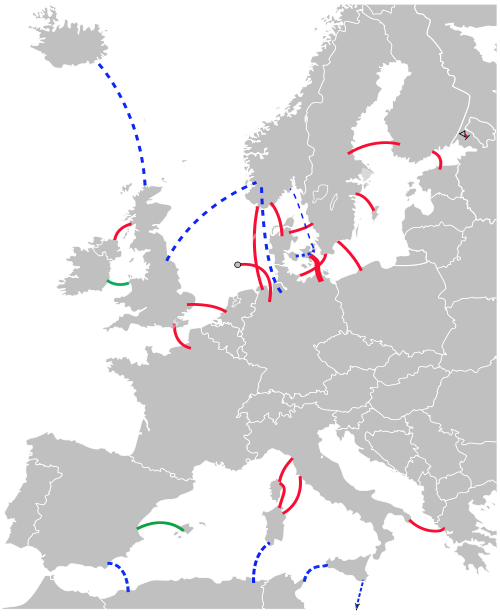
\includegraphics[scale=0.5]{HVDC_Europe.png}
\end{center}
\caption{HGÜ-Leitungen in Europa -- Rot: bestehend, Grün: in Bau; Blau: geplant. Quelle: \cite{Europa}}
\label{pic:Europa}
\end{figure}

In Europa ist der Einsatz von HGÜ jedoch immer noch fast ausschließlich auf Seekabel beschränkt -- auf allen anderen Kontinenten (natürlich ausgenommen der Antarktis) gibt es hingegen auch lange gleichstrombetriebene Freileitungen:

So wurde bereits 1979 die 1410 Kilometer lange HGÜ-Freileitung \q Cahora Bassa\qe zwischen der Cahora Bassa-Talsperre im Norden von Mosambik und dem Großraum um Johannesburg in Südafrika fertiggestellt (Spannung: $\pm$533 kV; Leistung: 1920 MW)
und im gleichen Jahr wurde auch eine 1770 Kilometer lange Freileitung \q Inga Shaba\qe in der heutigen Demokratische Republik Kongo (Spannung: $\pm$500 kV; Leistung: derzeit 200 MW, ausgelegt auf 560 MW) errichtet\cite{Schymroch}.
Auch \q Inga Shaba\qe dient zur Verteilung von Energie aus einem Wasserkraftwerk (Inga-Staudammes),
bei ihr wurden für die Pole jeweils eine eigene Trasse gebaut und sie kann sowohl bipolar als auch mono- oder homopolar betrieben werden\cite{Schymroch}.
In Nordamerika existieren zahlreiche HGÜ-Anlagen, besonders hervorzuheben ist unter anderem die HGÜ Quebec–New England, welche zwei asynchrone Netze über 1.500 Kilometer mit einer Übertragungsleistung von 2,25 GW verbindet und dabei 3 Stromrichterstationen hat (Spannung: $\pm$450 kV; errichtet 1986, ausgebaut 1992)\cite{Liste}.
Die mit über 2,500 km weltweit längste Freileitung soll noch dieses Jahr in Brasilien fertig gestellt werden, auch sie ist eine der wenigen Leitungen die drei Punkte verbindet (Spannung: $\pm$600 kV; Leistung: 3.150 MW). %cite
In Neuseeland wird ein beträchtlicher Teil der Energie der Nordinsel mit der bereits 1965 errichteten und zahlreich um- und ausgebauten Leitung \q Inter-Island\qe von der Südinsel bezogen (Spannung: +270 kV, -350 kV; Leistung: 1240 MW; Länge: 535 km Freileitung und 40 km Seekabel) \cite{Schymroch}\cite{Liste}.
In Asien setzen, wie auch schon angesprochen, vor allem China zahlreiche Gleichstromanlagen zum Ausbau des schnell wachsenden Stromnetzes ein, dies dürfte neben dem starken Wirtschaftswachstum auch in der enormen Größe des Landes begründet sein.

In den letzten Jahren erlebte die HGÜ-Technik durch den Boom der erneuerbaren Energien einen neuen Aufschwung, da diese zu stärkeren örtlichen und zeitlichen Unterschieden der Energieproduktion führen
So ist zum Beispiel in Norddeutschland, im Vergleich zu Süddeutschland, ein sehr großes Potential an Windkraft verfügbar. Daher planen deutsche Netzbetreiber laut Berichten der FAZ und der Financial Times Deutschland HGÜ-Trassen von Magdeburg ins Rhein-Main-Gebiet, von Rheinland nach Baden-Württemberg und von Schleswig-Holstein nach Bayern.\cite{FAZ1}\cite{FAZ2}\cite{FinancialTimes}
Durch diesen Aufschwung ist der Begriff der Hochspannungs-Gleichstrom-Übertragung auch außerhalb der Fachwelt deutlich bekannter geworden.

Besonders wichtig wäre eine Gleichstromübertragung auch für das DESERTEC-Konzept, welches vorsieht große Mengen an in Afrikanischen Wüsten erzeugten Ökostrom in die europäischen Energienetze einzuspeisen. Die Übertragung der Energie vom Afrikanischem zum europäischem Kontinent wäre nur mit HGÜs sinnvoll umsetzbar und auch innerhalb Europas bräuchte es HGÜ-Leitungen um die Redundanz, Stabilität und Versorgungssicherheit des Netzes zu gewährleisten.\cite{TRANS-CSP}

